\documentclass[../intro.tex]{subfiles}
\begin{document}
\section{Notation \& Definitions}
\begin{figure}
    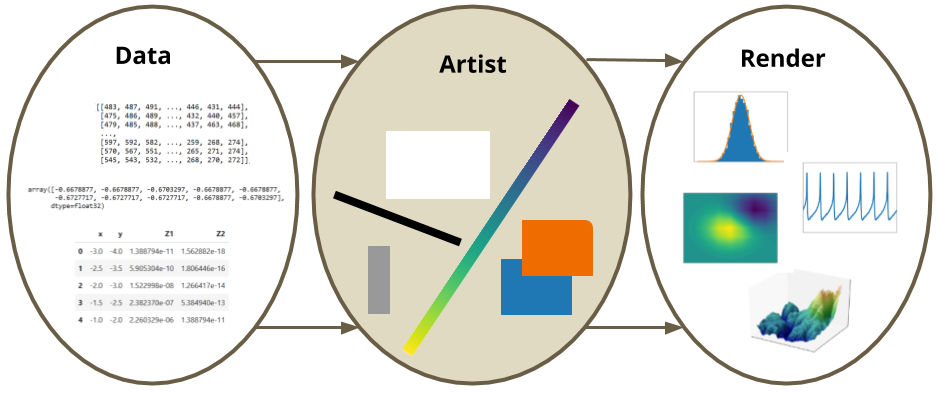
\includegraphics{figures/sections/dar.png}
    \caption{Data with semantic structure (such as tables and images) is mapped to visual encodings (color, position) that are composited into visual idioms (scatter, line) that are rendered into graphics (rasters, vectors).}
    \label{fig:artists}
\end{figure}
Figure~\ref{fig:artists} shows transformation from data into rendered graphical object, wherein there is an intermediate artist stage where the data gets transformed into a visual form. We argue that a faithful representation of the data is one where:
invariance:
functor
* types: variables measurement groups are  with visual encoding groups
* topology: visual idioms preserve the topology/connectivity of the dat


We propose that the mapping of a precise subset of data to a visual idiom ($I$) can be encapsulated in a class of functors called artists.
Gluing keys along a base space

\begin{equation}
    A: {\sigma \in \Gamma(V)}\mapsto f:\T \mapsto R^{7}
\end{equation}
diagram here: gamma is a dataframe, t is like xkcd line (clear abstract), R7 is nice pixelated version 
\begin{definition}
    \item[$F$] fiber, which is the space of all possible values encoded in the fiber bundle
    \item[$K$] base space, tells how the values in the fibers are connected, is analogous to the indexer in data containers
    \item[$V$] $F$ = $K \X F$ total space of the fiber bundle, which is space of all possible values on the index 
    \item[$\sigma(k)$] section of the fiber at a single k, (record on the  r) (dataframe)
    \item[$\Gamma(V)$] set of all possible sections (Spivak - $\Gamma(\sigma))$ - is space of all dataframes (we use this in artists to generalize- class of functions/sigmas that the artist can work on)
    \item[$f$] analogous to spec (such as svg or raster) that render will rely on to translate image to screen
    \item[$\T \in CW$] cw simplex representing topology of visual elements on screen (embedded in code rather than explicit) 
    \item[$R^{7}$]  {R,G,B,A, x, y, z} pixel in display space
\end{definition}

\begin{equation}
    A: {\sigma \in \Gamma(V)}\mapsto f:\T \mapsto R^{7}
\end{equation}

\subsubsection{Data}
We are using Butler's visualization model built on the mathematics of fiber bundles \cite{butlerVectorBundleClassesForm1992,butlerVisualizationModelBased1989} and Spivak's schema like description of fibers \cite{spivakSIMPLICIALDATABASES} as the basis of our data model. Fiber bundles give us a way to disentangle the connectivity of the data (is it a timeseries, a map?) from the variables in the dataset (temperature). Building on Munzner's formulation of the former as keys and the latter as values \cite{munznerWhatDataAbstraction2014}, the data has implicit keys that lie in the $K$ basespace of the fiberbundle, while the labels for the keys (such as latitude and longitude) are variables of the dataset that lie in the fiber $F$. 


%%%maybe this comes in a later API section....
\begin{center}
    \table{tab:fiberbundle}
    \begin{tabular}{ c c c }
     term & mathematical definition & data container analog\\
      $K$ & base space along which the data lies & indexer \\
      $F$ & fiber space from which possible values are pulled & schema \\
      $E$ & trivial: $F= K \times F$, non-trivial \dots & 
    \end{tabular}
\end{center}




\begin{figure}
    \lable{fig:simplex}
    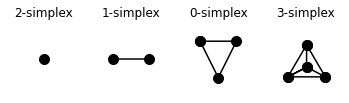
\includegraphics{figures/sections/math/simplex.png}
    \caption{Examples of simplexes that can be connected to make up a trivial total space $E = K\times F$.
    EX: data that both has a vertex & edge - find & visualize}
\end{figure}


In our data model, we encode the indexer as its simplex representation so that we can keep all variables of the fiber encoded on a simplex together \cite{butlerVisualizationModelBased1989}

trivial: 
locally trivial: take small enough regions, it becomes trivial, cutting it up into simplixes is one way to do so...
gluing maps are transition functions <- interesting things are in transition functions <- currently writing about pieces, they would write transition function validators and sections that we would check against
sheaf: association of u (point on eaerth) w/ its section (sheafs associates queries of data fibers over particular u)
pre-sheaf - just need space of sections for u
sheaf - if on section of u and section of v and they agree on intersection than their should be a section of union

\subsection{artist}
%%category theory diagrams to show artist is a functor, which is how you get invariance
%% artist is parameterized on taus
%% artists are curried collection of taus , orbits of artists are the visual idiomsW
\begin{equation}
    A: \sigma \in \Gamma(V), \Taus \mapsto f:\T \mapsto R^{7}
\end{equation}
$\sigma$ evaluated on $k \in K$
%%%in practuce this has currently same topology as gamma V
\begin{equation}%%pull in spivak
    \tau: one type in the fiber \mapsto different type in the T fiber 

\subsection{render}
\begin{equation}
    f: \T \mapsto R^{7}
\end{equation}

\end{document}